\paragraph{Question resampling changes the endpoint decision.}
On 400 untouched HotpotQA questions, guarded FBG reaches 24.75 EM versus
24.50 for the full budget. The paired difference is $+0.25$ with a 95\%
interval of $[-0.75,1.50]$ and a one-sided lower bound of $-0.75$. Calls fall
from 9.00 to 6.75, input tokens fall by 30.7\%, output tokens by 27.1\%, and
wall time by 23.8\%. The endpoint therefore passes the declared 3-EM
non-inferiority and call-reduction rule. The two-sided interval contains zero,
so the matched-cost and replication analyses determine the stronger claim.

\begin{figure}[t]
  \centering
  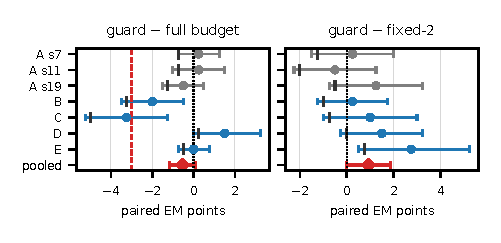
\includegraphics[width=\columnwidth]{figures/fig_samples_main.pdf}
  \caption{Guarded FBG minus full search or two fixed searches. Grey rows rerun
  HotpotQA sample A with new seeds, and blue rows are new question samples.}
  \label{fig:samples}
  \Description{Forest plot of paired exact-match differences between guarded
  FBG and full search or two fixed searches. Each row is one run. Bars show 95 percent
  intervals, ticks show one-sided lower bounds, and a dashed line marks the
  negative three point margin.}
\end{figure}

Figure~\ref{fig:samples} separates decoding and population variation. With the
same 400 questions, decoding seeds 7, 11, and 19 give guarded differences of
$+0.25$, $+0.25$, and $-0.50$ EM. All pass the predeclared rule. Four new
question draws give $-2.00$, $-3.25$, $+1.50$, and $0.00$ EM. Their one-sided
lower bounds are $-3.25$, $-5.00$, $+0.25$, and $-0.50$, so two of four pass
and two fail. Across all five question samples, three of five pass. The two
negative cellwise intervals do not remain directional under the max-t
family-wise band. The draw disagreement is the substantive result because it
overturns the stable decision suggested by same-question decoding reruns.

The draw-level mean is $-0.70$ EM with one-sided lower bound $-2.51$. Pooled
contrasts against full search and fixed-3 are $-0.54$ $[-1.18,0.11]$ and
$-0.32$ $[-1.03,0.37]$ EM, and both contain zero. Contrasts favoring the guard over fixed-2 or repetition use
1.67 and 0.90 more calls. Thus every favorable pooled contrast costs more,
while every equal-cost or lower-cost contrast remains unresolved.

Between-draw contrast variation is larger than the same-question decoding
variation in this small panel. With five question draws and three decoding
seeds, we do not estimate a stable variance decomposition. Descriptively,
$I^2=80\%$ is the share of observed heterogeneity beyond within-draw
uncertainty, while $\tau=1.25$ EM is the estimated between-draw standard
deviation. Neither is a population parameter in this five-draw panel. Only 44
of 2{,}000 questions produce different full-budget and guarded answers, so a
small item set can determine a draw-level decision.

\paragraph{Backbone crosses and Wikipedia-derived datasets.}
Three Claude Haiku 4.5 draws with $n=200$ and one Llama-3.2-3B draw with
$n=400$ all pass the 3-EM margin. Guarded FBG reaches the pooled frontier in
none, and its mean equal-call difference is $+0.14$ EM. Changing the backbone
therefore changes the accuracy level more than the deployment verdict.

On the 25{,}247{,}888-sentence FEVER Wikipedia index, guarded FBG has paired
difference $-0.25$ EM with interval $[-2.00,1.25]$ and lowers calls from 9.00
to 5.90. Fixed-2 still dominates it. Three 2Wiki draws lower calls to between
5.5 and 5.7, but fixed-2 dominates the guard in every draw. On three MuSiQue
draws, answer repetition or fixed-2 also dominates the guard. The repeated
domination extends the result beyond one Wikipedia-derived benchmark. We
interpret these cells as related environments because they share a sparse
retrieval stack and multi-hop task design.

\paragraph{One external news-corpus cell.}
We froze one MultiHopRAG inference-query cell before fitting or test
evaluation. It contains 400 questions over 609 English news articles and uses
Qwen2.5-3B with the same four-search cap. Table~\ref{tab:external-policies}
separates the frozen FBG endpoint from three exploratory signal policies. Each
gain compares a policy to the randomized simple hull at equal
mean calls.

\begin{table}[H]
\caption{External news-cell policies at equal calls to the simple-policy hull.}
\label{tab:external-policies}
\footnotesize
\setlength{\tabcolsep}{8.4pt}
\rowcolors{2}{rowshade}{}
\begin{tabular}{@{}lrrrl@{}}
\toprule
\hiderowcolors
\tabhead \textbf{Policy} & \textbf{EM} & \textbf{Calls} & \textbf{Gain vs.\ simple} & \textbf{95\% CI} \\
\midrule
\showrowcolors
FBG-only & 73.00 & 7.27 & $+0.48$ & $[-0.50,1.46]$ \\
Guarded FBG & 73.25 & 7.40 & $+0.71$ & $[-0.07,1.57]$ \\
Stop classifier & 70.50 & 4.35 & $+2.10$ & $[0.12,4.10]$ \\
Error-head gate & 73.75 & 7.65 & $+1.18$ & $[0.41,2.06]$ \\

\bottomrule
\end{tabular}
\end{table}

Guarded FBG reaches 73.25 EM at 7.40 calls, compared with 72.75 EM at 9.00
calls for full search. It passes the declared endpoint, but the
matched-cost advantage remains unresolved. The binary future-improvement and
error-head intervals are positive, yet both policies are exploratory and come
from one question draw.
The cell therefore shows that the signal choice can change a boundary result.
As a single draw with a per-cell refitted head, it does not establish
cross-domain controller transfer.
